\section{Choice of Optimization Objective}

\subsection{Regression}
When faced with the challenge of estimating discrete ordinal quantities, such as the number of sources in model order estimation tasks,
the initial inclination might lean towards employing regression models.
At first glance, these models offer a straightforward approach, potentially allowing for the interpretation of their
quasi-continuous output as a discrete source count after appropriate rounding.\\
However, this method exhibits intrinsic limitations due to the absence of inherent output bounds in regression models,
leading to the necessity for artificial scaling interventions.

Solutions like applying a scaled sigmoid function to the regression layer's output have been contemplated to confine the
predictions within the required range of \( [0, N_{\max}] \).\\
Despite its theoretical viability, this approach inadvertently biases the model towards mid-range values,
complicating the differentiation between adjacent classes, especially at the boundary values.

A more feasible alternative is to transform the output of the regression layer according, would be to round it to
the nearest integer and clamp it, such that it falls within the valid range of source counts.
% Add a brief explanation of ˜\hat{bfm{y}}_reg˜ - single neuron output -> #Params in regression layer: # CHs_prev_layer * 1
\begin{equation}
    \bfm{\NPred}_{\text{reg}} = \max\left(0,\:\min(N_{\max},\:\nint{\hat{\bfm{y}}})\right), \quad \hat{\bfm{y}} \in \mathbb{R}^{\B}, \: \bfm{\NPred}_{\text{reg}} \in \NSet^{\B}
    \label{eq:regression_clamp}
\end{equation}

Similarly to~\cite{yang2020} we decided to employ the \gls{mse} (\( \mathcal{L}_2 \)) loss function for the regression model.
\begin{equation}
    \lossMSE(\hat{\bfm{y}}, \bfm{N}) = \frac{1}{\B} \sum_{i=1}^{\B} \left(\hat{y}_i - N_i\right)^2, \quad \hat{y}_i \in \mathbb{R},\: N_i \in \NSet
    \label{eq:mse_loss}
\end{equation}

\subsection{Classification}
For convenience, let \( C \coloneq N_{\max} + 1 = \| \NSet \| \) denote the number of classes in the classification task.\\
The classification approach provides a more intuitive and efficient solution to the task. Rather than using a regression
layer with a single neuron output, we utilize a classification layer that produces a tensor of logits \( \bfm{Z} \in \mathbb{R}^{\B \times C}\).
This enables the classification model to have separate output units for each class.\\
To denote the logits vector for a specific sample within the batch, let \( \bfm{z} \coloneq \bfm{Z}_{b,:} \),
where \( \bfm{z} \in \mathbb{R}^{C} \) represents the logits for the \( b \)-th sample across all \( C \) classes.\\
The interpretation of each element within the logits vector \( \bfm{z} \) corresponds to the log-likelihood for class
memberships, where \( z_c = \ln \Pr(N=c|\bfL; \bfm{\omega}) \) represents the logarithm of the probability that
the model order \( N \) equals class \( c \), conditioned on the input \( \bfL \) and parameterized by the model weights
\( \bfm{\omega} \)~\cite[Chapter 6]{dlbook}.

During inference, the model order estimate \( \NPred_{\text{cls}} \) is obtained by determining the index of the maximum element in
the logits vector \( \bfm{z} \):
\begin{equation}
    \bfm{\NPred}_{\text{cls}} = \argmax_{c \in \NSet} \bfm{Z}_{:,c}, \quad \bfm{\NPred}_{\text{cls}} \in \NSet^{\B}
    \label{eq:classification_argmax}
\end{equation}

For the purpose of training, however, the softmax activation function is applied to the logits, converting them into a valid probability
distribution across the class labels. The transformation \( \mathrm{softmax} : \mathbb{R}^C \rightarrow [0, 1)^C \) is defined by:
\begin{equation}
    \hat{y}_c = \text{softmax}(\bfm{z})_c = \frac{e^{z_c}}{\sum_{j=1}^{C} e^{z_j}}, \quad c \in \NSet
    \label{eq:softmax}
\end{equation}
where \(\hat{y}_c\) represents the predicted probability that the model assigns to class \(c\), given the logits
vector \(\bfm{z}\) for a specific sample. The softmax function ensures that the output probabilities sum to one,
facilitating a direct comparison with the true class labels.

Consequently, the cross-entropy loss function is utilized to quantify the discrepancy between the predicted probability
distribution and the true label distribution and is defined as follows:
\begin{equation}
    \lossCE(\hat{\bfm{Y}}, \dot{\mbf{Y}}_N) = -\frac{1}{\B} \sum_{b=1}^{\B} \sum_{j=1}^{C} N_{bj} \ln(\hat{y}_{bj}), \quad \dot{\mbf{Y}}_N, \hat{\bfm{Y}} \in \mathbb{R}^{\B \times C}
    \label{eq:ce_loss}
\end{equation}
In \autoref{eq:ce_loss}, \( \dot{\mbf{Y}}_N \) represents the true class labels in one-hot encoding. Each row of \( \hat{\bfm{Y}} \),
denoted as \( \hat{\bfm{y}} = [\hat{y}_1, \ldots, \hat{y}_c] \), represents the model's predicted probabilities for a particular sample.

\subsection{Comparison and Conclusion}

\begin{figure}[H]
    \centering
    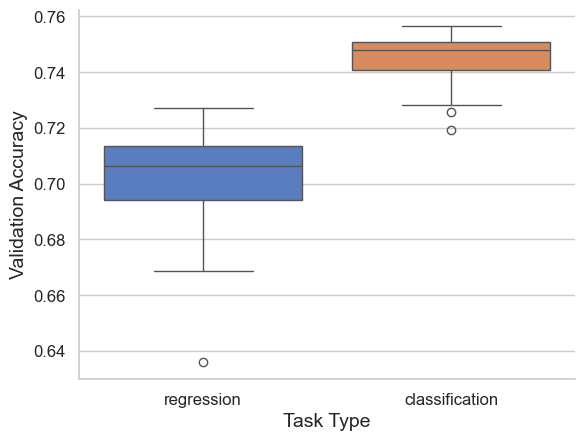
\includegraphics[width=0.45\textwidth]{figures/06_ModelExploration/conv_task_type.png}
    \caption{Boxplot of \( \meanAccVal \) for the regression and classification tasks.}
    \label{fig:task_type}
\end{figure}

Figure~\ref{fig:task_type} compellingly demonstrates the superior performance of the classification paradigm over
regression in terms of validation accuracy. A brief explanation of the employed boxplots is provided in~\autoref{app:sec:Boxplot}.
To quantify this advantage,~\autoref{tab:accuracy_change} details the relative improvement when switching from regression
to classification.

\begin{table}[H]
    \centering
    \caption{Quantitative Performance Metrics: Regression vs. Classification}
    \label{tab:accuracy_change}
    \begin{tabular}{@{}lcc@{}}
    \toprule
    & \multicolumn{2}{c}{\( \meanAccVal \)} \\
    \cmidrule(lr){2-3}
    Task Type & \( \nu \) & \( \%\Delta \) \\
    \midrule
    Regression~\bigoplus~\( \lossMSE \) & 0.7062 & — \\
    Classification~\bigoplus~\( \lossCE \) & 0.7478 & \gnbx{+5.889\%} \\
    \bottomrule
    \end{tabular}
\end{table}

The data presented in \autoref{tab:accuracy_change} as well as the boxplots in \autoref{fig:task_type} were obtained by optimizing for
the respective loss functions \( \lossMSE \) and \( \lossCE \) on the validation set \( \DMain_{(\text{val})} \) using an
earlier the \gls{cnn} architecture, which will be introduced in \autoref{sec:cnn}.


The only downside of employing the classification approach is an increase in computational cost due to the
additional \( C - 1 \) neurons in the output layer. Assuming a total of \( K_{\text{CH}} \) channels or features in the
previous layer, the number of parameters in the output layer for both tasks given by:
\begin{align}
    \#\text{Params}_{\text{head,reg}} &= K_{\text{CH}} \times 1 \\
    \#\text{Params}_{\text{head,cls}} &= K_{\text{CH}} \times C
\end{align}

This increased computational cost is a small price to pay for the significant improvement in performance, which is
why we decided to proceed with the classification approach for the remainder of the study. Both, the softmax activation
function and the multi-class cross-entropy loss function are embedded into the categorical cross-entropy loss function
that is provided by the \textsc{PyTorch} library.

Given the applicability of cost functions like \gls{mse} \( \loss^{\text{MSE}} \) regardless of the task type, it might
be worthwhile to explore the use of \gls{mse} or a similar loss function with an emphasis on the regressive nature of
the output, in a hybrid approach in combination with the softmax \( \oplus \) cross-entropy loss.
